\documentclass{article}
\usepackage{amsmath}
\usepackage{amssymb}
\usepackage{graphicx}
\usepackage{hyperref}
\usepackage[version=4]{mhchem}

\title{Example 17}
\date{}

\begin{document}
\maketitle

Triangle \(A B C\) is an isosceles triangle. \(D\) is on \(A B\). Extend \(A C\) to \(E\) and connect \(D E\) so that \(B D=C E\). Prove: \(D F=F E\).

Proof:
Draw \(D G \perp B C\), extend \(B C\), and then draw \(E H\) to meet the extension of \(B C\) at \(H\) such that \(E H \perp B C\).\\
\centering
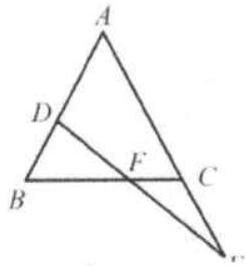
\includegraphics[width=\textwidth]{images/problem_image_1.jpg}

We see that \(D B=B E, \angle B=\angle A C B=\angle E C H, \angle D G B=\) \(\angle E H C=90^{\circ}\). Thus \(\triangle D B G \cong \triangle E H C\).\\
So \(D G=E H\).\\
\centering
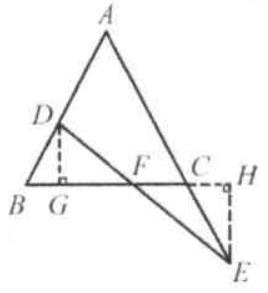
\includegraphics[width=\textwidth]{images/reasoning_image_1.jpg}


In \(\triangle D G F\) and \(\triangle E H F, \angle G D F=\angle H E F\) (alternate interior angles of parallel lines of \(D G\) and \(E H), \angle D G F=\angle E H F=90^{\circ}, D G=E H\). Thus \(\triangle D G F \cong \triangle E H F\) and \(D F\) \(=E F\).


\end{document}
